\begin{frame}{Markov Chain}
\begin{center}
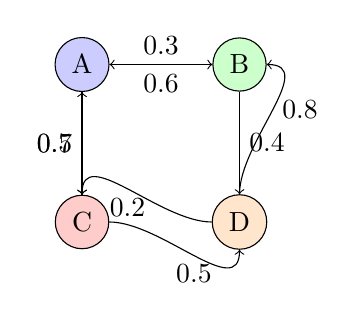
\begin{tikzpicture}[node distance=2cm]
    \node[circle, draw, fill=blue!20] (A) {A};
    \node[circle, draw, fill=green!20, right of=A] (B) {B};
    \node[circle, draw, fill=red!20, below of=A] (C) {C};
    \node[circle, draw, fill=orange!20, below of=B] (D) {D};
    
    \draw[->] (A) to[out=0,in=180] node[above] {0.3} (B);
    \draw[->] (A) to[out=270,in=90] node[left] {0.7} (C);
    \draw[->] (B) to[out=270,in=90] node[right] {0.4} (D);
    \draw[->] (B) to[out=180,in=0] node[below] {0.6} (A);
    \draw[->] (C) to[out=0,in=270] node[below] {0.5} (D);
    \draw[->] (C) to[out=90,in=270] node[left] {0.5} (A);
    \draw[->] (D) to[out=90,in=0] node[right] {0.8} (B);
    \draw[->] (D) to[out=180,in=90] node[below] {0.2} (C);
\end{tikzpicture}
\end{center}

\footnotesize
Markov chain with transition probabilities
\end{frame}